\chapter{Par\'ametros relacionados con la simulaci\'on computacional}
\label{sec-validation}
La validaci\'on posee una importancia crucial en el proceso de concepci\'on de un modelo matem\'atico-computacional pues constituye la verificaci\'on de su robustez, de su capacidad predictiva y de la veracidad de las hip\'otesis planteadas. Entre los distintos temas que se deben abordar en esta secci\'on se encuentran el an\'alisis de los valores asignados a los par\'ametros del modelo y las repercusiones de sus posibles variaciones, mientras que la comparaci\'on de los resultados num\'ericos y visuales obtenidos con datos provenientes de distintas investigaciones \textit{in vitro}, \textit{in vivo} y estudios cl\'inicos se realizar\'a en la secci\'on~\ref{sec-results}. Una configuraci\'on de la simulaci\'on comprende todos los par\'ametros cuyos valores son requeridos para la ejecuci\'on del aut\'omata celular. Es importante destacar que la totalidad del modelo est\'a concebido para reproducir el desarrollo de cualquier tipo de carcinoma, pero como se podr\'a apreciar en las secciones restantes nos concentramos en el carcinoma ductal infiltrante que constituye el caso m\'as frecuente del c\'ancer de mama. Entre las razones detr\'as de la elecci\'on est\'a la mayor abundancia de informaci\'on y datos respecto a este tipo de c\'ancer.

\section{Par\'ametros de la construcci\'on de la red y de la ley de crecimiento log\'istico}
\label{subsec-network-param}
Los par\'ametros de construcci\'on de la red se corresponden con los argumentos del algoritmo~\ref{alg-watts} mostrado en la secci\'on~\ref{subsec-watts-2}, y determinan el tama\~no del espacio que se utiliza para representar las localizaciones donde se desarrolla el c\'ancer. Se presentan en el cuadro~\ref{table-network-params} que aparece a continuaci\'on para una r\'apida referencia. Los par\'ametros de la ley de crecimiento log\'istico se utilizan para reproducir el crecimiento tumoral, espec\'ificamente en las reglas presentadas en las secciones~\ref{subsec-celldiv} y \ref{subsec-micrometastasis} obtenidas a trav\'es de un proceso de inferencia de la regla a partir de dicha ley continua. Se presentan en el cuadro~\ref{table-logistic-params} para una r\'apida referencia.

\begin{table}[!ht]
\begin{center}
\scalebox{0.9}{\begin{tabular}{|p{2cm}|p{14.5cm}|} \hline
\emph{Par\'ametro} & \emph{Descripci\'on} \\\hline
\multicolumn{1}{|c|}{$s_x$, $s_y$} & Dimensiones del espacio declarado. Las componentes espaciales de los v\'ertices del grafo poseen los siguientes rangos de valores: $0 \leq x < s_x$ y $0 \leq y < s_y$. \\\hline
\multicolumn{1}{|c|}{$s_o$} & Valor que marca la divisi\'on de la red entre un \'organo y el otro. Posee el siguiente rango de valores: $0 \leq s_o < s_x$. Generalmente toma valor $s_o = s_x / 2$. \\\hline
\multicolumn{1}{|c|}{$p$} & Probabilidad de reconexi\'on del modelo Watts-Strogatz. \\\hline
\end{tabular}}\vspace*{-0.5cm}
\end{center}
\caption[Par\'ametros de la construcci\'on de la red utilizados por el modelo Watts-Strogatz]{Par\'ametros de la construcci\'on de la red utilizados por el modelo Watts-Strogatz.}
\label{table-network-params}
\end{table}

\begin{table}[!ht]
\begin{center}
\scalebox{0.9}{\begin{tabular}{|p{2cm}|p{14.5cm}|} \hline
\emph{Par\'ametro} & \emph{Descripci\'on} \\\hline
\multicolumn{1}{|c|}{$P_0^a$, $P_0^v$} & Poblaciones iniciales de las etapas avascular y vascular respectivamente. \\\hline
\multicolumn{1}{|c|}{$r_a$, $r_v$} & Ritmos de proliferaci\'on de las etapas avascular y vascular respectivamente. \\\hline
\multicolumn{1}{|c|}{$K_a$, $K_v$} & Capacidad de carga de las etapas avascular y vascular respectivamente. \\\hline
\multicolumn{1}{|c|}{$\Delta t$} & Tiempo transcurrido entre los instantes de tiempo $n$ y $n+1$. \\\hline
\multicolumn{1}{|c|}{$n_a$} & Tiempo que permanece un tumor en etapa avascular. \\\hline
\end{tabular}}\vspace*{-0.5cm}
\end{center}
\caption[Par\'ametros correspondientes con la ley de crecimiento log\'istico]{Par\'ametros correspondientes con la ley de crecimiento log\'istico.}
\label{table-logistic-params}
\end{table}

En la secci\'on~\ref{subsec-macro} se expuso que un tumor avascular solo puede crecer hasta un radio de $R_a \in [0$.$5, 1]mm$. Asumiendo que un tumor tiene forma esf\'erica se estima que el volumen ocupado por el mismo durante la etapa avascular posee un valor perteneciente al intervalo $V_a \in [0$.$5236, 4$.$189]mm^3$. En~\cite{breastdata,chile} se estima que el radio de un tumor vascular correspondiente con un carcinoma ductal infiltrante puede tener valores de $R_v \in [10, 15]mm$. Siguiendo la idea anterior se estima que el volumen ocupado por un tumor vascular de estas dimensiones posee un valor perteneciente al intervalo $V_v \in [4$.$189 \times 10^3, 1$.$414 \times 10^4]mm^3$. El radio de una c\'elula cancer\'igena toma un valor del siguiente intervalo $R_c \in [1$.$5 \times 10^{-2}, 2$.$0 \times 10^{-2}]mm$ tomando en cuenta los tipos m\'as comunes de carcinomas~\cite{kansal3,breastdata,vajtai}. En~\cite{wisconsin} este valor se estima en $R_c \approx 17$.$46 \mu m$, utilizando en el c\'alculo $212$ muestras de c\'elulas obtenidas de tumores del tipo carcinoma ductal infiltrante, que constituye la forma m\'as com\'un de c\'ancer de mama. Asumiendo que una c\'elula tiene forma esf\'erica se determina su volumen aproximado como $V_{c} \in [1$.$414 \times 10^{-5}, 3$.$351 \times 10^{-5}]mm^3$. Utilizando los intervalos de valores del volumen de la c\'elula cancer\'igena y de un tumor durante las etapas avascular y vascular se pueden determinar las capacidades de carga del entorno para ambas etapas, devolviendo los siguientes intervalos $K_a \in [1$.$563 \times 10^4, 2$.$963 \times 10^5]$ y $K_v \in [1$.$25 \times 10^8, 1$.$0 \times 10^9]$. 

Los intervalos de valores antes mencionados son los que se requieren para una simulaci\'on que se lleve a cabo en tres dimensiones, pero dado que el presente modelo solo utiliza dos de estas, es necesario realizar una serie de transformaciones adicionales. Como se expres\'o en la hip\'otesis XII sobre la representaci\'on del tejido el modelo se concibe como una reproducci\'on de un corte de tejido como se aprecia en la figura~\ref{fig-transformation}. Se infiere que se debe asumir que dicho corte se corresponde con una circunferencia con radio igual al del tumor en cualquiera de sus etapas. De esta forma tenemos que el \'area ocupada por un tumor avascular pertenece al intervalo $A_a \in [7$.$854 \times 10^{-1}, 3$.$142]mm^2$ y el de un tumor vascular pertenece al intervalo $A_v \in [3$.$142 \times 10^2, 7$.$069 \times 10^2]mm^2$. Siguiendo el mismo an\'alisis se asume que una secci\'on de una c\'elula posee una forma semejante a una circunferencia, por lo que utilizando el radio de una c\'elula cancer\'igena se puede obtener la superficie ocupada por dicha secci\'on, devolviendo un valor que pertenece al intervalo $A_c \in [7$.$069 \times 10^{-4}, 1$.$257 \times 10^{-3}]mm^2$. Finalmente, las capacidades de carga para las etapas avascular y vascular poseen valores que pertenecen a los intervalos $K_a \in [6$.$25 \times 10^2, 4$.$444 \times 10^3]$ y $K_v \in [2$.$5 \times 10^5, 1$.$0 \times 10^6]$. En el cuadro~\ref{table-original-values} aparecen recogidos los datos mencionados anteriormente para una r\'apida referencia.

\begin{figure}[!ht]
\begin{center}
\scalebox{0.45}{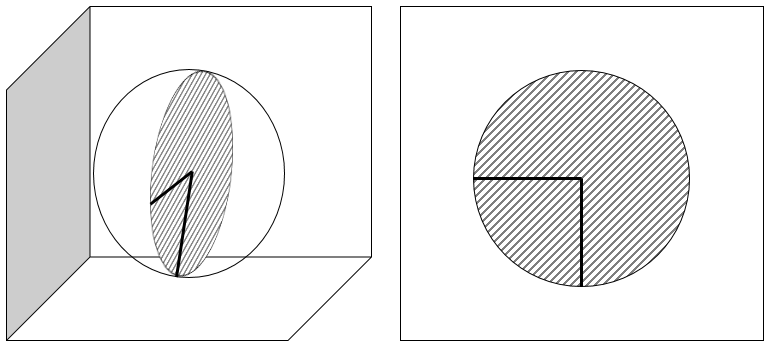
\includegraphics{img/transformation.png}}
\end{center}\vspace*{-0.75cm}
\caption[Transformaci\'on de la representaci\'on de un tumor en tres dimensiones a dos dimensiones]{Transformaci\'on de la representaci\'on de un tumor en tres dimensiones a dos dimensiones. Se observa el uso de la secci\'on o corte de la esfera que presenta mayor \'area.}
\label{fig-transformation}
\end{figure}

\begin{table}[!ht]
\begin{center}
\scalebox{0.9}{\begin{tabular}{|c|c|c|c|c|} \hline
\multicolumn{2}{|c|}{\emph{Datos}} & \multicolumn{1}{|l|}{\emph{M\'inimo}} & \multicolumn{1}{|l|}{\emph{M\'aximo}} & \multicolumn{1}{|l|}{\emph{Promedio}}\\\hline

 & \multicolumn{1}{|l|}{$R_c(mm)$} & \multicolumn{1}{|c|}{$1$.$5 \times 10^{-2}$} & \multicolumn{1}{|c|}{$2$.$0 \times 10^{-2}$} & \multicolumn{1}{|c|}{$1$.$75 \times 10^{-2}$} \\\cline{2-5}                              
\emph{C\'elula cancer\'igena} & \multicolumn{1}{|l|}{$V_c(mm^3)$} & \multicolumn{1}{|c|}{$1$.$414 \times 10^{-5}$} & \multicolumn{1}{|c|}{$3$.$351 \times 10^{-5}$} & \multicolumn{1}{|c|}{$2$.$2244 \times 10^{-5}$} \\\cline{2-5} 
 & \multicolumn{1}{|l|}{$A_c(mm^2)$} & \multicolumn{1}{|c|}{$7$.$069 \times 10^{-4}$} & \multicolumn{1}{|c|}{$1$.$257 \times 10^{-3}$} & \multicolumn{1}{|c|}{$9$.$621 \times 10^{-4}$} \\\hline
                              
 & \multicolumn{1}{|l|}{$R_a(mm)$} & \multicolumn{1}{|c|}{$0$.$5$} & \multicolumn{1}{|c|}{$1$} & \multicolumn{1}{|c|}{$7$.$5 \times 10^{-1}$} \\\cline{2-5}
 & \multicolumn{1}{|l|}{$V_a(mm^3)$} & \multicolumn{1}{|c|}{$5$.$236 \times 10^{-1}$} & \multicolumn{1}{|c|}{$4$.$189$} & \multicolumn{1}{|c|}{$1$.$767$} \\\cline{2-5} 
\emph{Tumor avascular} & \multicolumn{1}{|l|}{$K_a$*} & \multicolumn{1}{|c|}{$1$.$563 \times 10^4$} & \multicolumn{1}{|c|}{$2$.$963 \times 10^5$} & \multicolumn{1}{|c|}{$7$.$872 \times 10^4$} \\\cline{2-5} 
 & \multicolumn{1}{|l|}{$A_a(mm^2)$} & \multicolumn{1}{|c|}{$7$.$854 \times 10^{-1}$} & \multicolumn{1}{|c|}{$3$.$142$} & \multicolumn{1}{|c|}{$1.767$} \\\cline{2-5} 
 & \multicolumn{1}{|l|}{$K_a$**} & \multicolumn{1}{|c|}{$6$.$25 \times 10^2$} & \multicolumn{1}{|c|}{$4$.$444 \times 10^3$} & \multicolumn{1}{|c|}{$1$.$837 \times 10^3$} \\\hline
					   
 & \multicolumn{1}{|l|}{$R_v(mm)$} & \multicolumn{1}{|c|}{$1$.$0 \times 10^1$} & \multicolumn{1}{|c|}{$1$.$5 \times 10^1$} & \multicolumn{1}{|c|}{$1$.$25 \times 10^1$} \\\cline{2-5}
 & \multicolumn{1}{|l|}{$V_v(mm^3)$} & \multicolumn{1}{|c|}{$4$.$189 \times 10^3$} & \multicolumn{1}{|c|}{$1$.$414 \times 10^4$} & \multicolumn{1}{|c|}{$8$.$181 \times 10^3$} \\\cline{2-5} 
\emph{Tumor vascular} & \multicolumn{1}{|l|}{$K_v$*} & \multicolumn{1}{|c|}{$1$.$25 \times 10^8$} & \multicolumn{1}{|c|}{$1$.$0 \times 10^9$}& \multicolumn{1}{|c|}{$3$.$644 \times 10^8$} \\\cline{2-5} 
 & \multicolumn{1}{|l|}{$A_v(mm^2)$} & \multicolumn{1}{|c|}{$3$.$142 \times 10^2$} & \multicolumn{1}{|c|}{$7$.$069 \times 10^2$} & \multicolumn{1}{|c|}{$4$.$909 \times 10^2$}\\\cline{2-5} 
 & \multicolumn{1}{|l|}{$K_v$**} & \multicolumn{1}{|c|}{$2$.$5 \times 10^5$} & \multicolumn{1}{|c|}{$1$.$0 \times 10^6$} & \multicolumn{1}{|c|}{$5$.$102 \times 10^5$}\\\hline
\end{tabular}}\vspace*{-0.5cm}
\end{center}
\caption[Datos de las caracter\'isticas f\'isicas como el radio y vol\'umen de la c\'elula cancer\'igena, de un tumor en etapa avascular y vascular, y de la superficie que ocupa un corte transversal de los mismos]{Datos de las caracter\'isticas f\'isicas como el radio y vol\'umen de la c\'elula cancer\'igena, de un tumor en etapa avascular y vascular, y de la superficie que ocupa un corte transversal de los mismos, correspondientes con el tipo de c\'ancer de mama conocido como carcinoma ductal infiltrante. \emph{En el cuadro:} (*) Capacidad de carga con respecto al volumen; (**) Capacidad de carga con respecto a la superficie ocupada por el corte transversal.}
\label{table-original-values}
\end{table} 

Las localizaciones donde se reproduce el ciclo vital tumoral deben poseer el espacio suficiente para contener varias lesiones neopl\'asicas, motivo por el que se representa un corte de tejido de dimensiones $[0,10]cm \times [0,5]cm$, donde las porciones $[0,5]cm \times [0,5]cm$ y $[5,10]cm \times [0,5]cm$ se corresponden con el \'organo primario y secundario respectivamente. Las dimensiones de este espacio con respecto al n\'umero de c\'elulas contenidas se estima mediante el radio promedio de una c\'elula cancer\'igena $R_c$, quedando un espacio de dimensiones $[0, 3000] \times [0, 1500]$ aproximadamente, para un total de $4$.$5 \times 10^6$ c\'elulas. Por tanto, los par\'ametros de construcci\'on de la red de las dimensiones del espacio declarado poseen los siguientes valores $s_x = 3000$ y $s_y = 1500$, mientras que la divisi\'on entre los \'organos es $s_o = 1500$. Como se expuso en la secci\'on~\ref{subsec-watts-2} la probabilidad de reconexi\'on de la red posee el siguiente rango de valores $p \in [10^{-3},10^{-2}]$.

Los par\'ametros que restan por definir son los ritmos de proliferaci\'on tumoral $r_a$ y $r_v$, y la cantidad de tiempo que transcurre entre el instante de tiempo $n$ y el $n+1$, o sea $\Delta t$. Los valores de estos par\'ametros espec\'ificos a la ley de crecimiento log\'istico no han sido analizados hasta este momento en ning\'un trabajo previo, por lo que sus valores ser\'an estimados con el objetivo de ajustar el comportamiento del aut\'omata celular y que reproduzca en la mayor medida posible los procesos que lleva a cabo el c\'ancer en la realidad. En la secci\'on~\ref{subsec-celldiv} se llev\'o a cabo un procedimiento que ten\'ia como objetivo lograr que los valores de la probabilidad de crecimiento tumoral, mostrados en las expresiones~(\ref{eq-pa}) y~(\ref{eq-pv}), estuviese acotada en el intervalo $[0,\rho_{max}]$, donde $\rho_{max}$ es un valor de probabilidad m\'aximo seleccionado a priori y que funciona como un mecanismo de ajuste. En~\cite{ruben} el valor m\'aximo alcanzado por la probabilidad de crecimiento tumoral es de aproximadamente $0$.$63$, mientras que en~\cite{kansal,kansal3} esta probabilidad var\'ia entre $0$.$192$ y $0$.$384$, lo cual nos otorga una medida para ajustar nuestra funci\'on de probabilidad. Este procedimiento culmin\'o con la obtenci\'on de la expresi\'on n\'umero~(\ref{eq-cond-1}) que asegura que dicha distribuci\'on de probabilidad est\'e acotada en el intervalo mencionado, pero que ofrece una metodolog\'ia para estimar los valores de $r_a$ y $r_v$. Seg\'un dicha condici\'on:
\begin{subequations}
\begin{equation*}
r_a \in \left[0, \frac{4 \rho_{max}^a}{K_a}\right],~r_v \in \left[0, \frac{4 \rho_{max}^v}{K_v}\right],
\end{equation*}
\end{subequations}
donde los valores de $K_a$ y $K_v$ fueron determinados anteriormente. El valor m\'aximo alcanzable de probabilidad se obtiene al hacer $\rho_{max}^a= K_a r_a / 4 = 1$ y $\rho_{max}^v= K_v r_v / 4 = 1$, que a su vez se obtiene cuando~(\ref{eq-cond-t}):
\begin{equation}
t = \frac{1}{r} \ln\frac{K-P_0}{P_0}
\end{equation}
donde si hacemos $t=n\Delta t$ obtenemos:
\begin{equation}
n = \frac{1}{r\Delta t} \ln\frac{K-P_0}{P_0}. \label{final}
\end{equation}

De esta expresi\'on~(\ref{final}) se infiere que el $\Delta t$ determina el punto donde la distribuci\'on de probabilidad alcanza su m\'aximo, dato relevante ya que esta distribuci\'on posee una curva semejante a la funci\'on gaussiana. De esta forma si conocemos el tiempo total que ocupa las etapas avascular o vascular dentro del ciclo de vida del tumor es posible ajustar esta distribuci\'on a los incrementos de tama\~no que presenta un tumor en ambas etapas. Se hace que el valor de $\Delta t$ se corresponda con un tiempo de $24$ horas. De esta forma el n\'umero de generaciones del aut\'omata coincide con la cantidad de d\'ias que est\'a simulando. En las gr\'aficas~\ref{graph-probability-distribution-avascular} se muestran las distribuciones de probabilidad de las funciones $\rho_a(n\Delta t)$~(\ref{eq-pa}) y $\rho_v(n\Delta t)$~(\ref{eq-pv}) que describen el crecimiento tumoral durante las etapas avascular y vascular respectivamente, tomando como lapso de tiempo $365$ d\'ias para ambas etapas. Como se puede apreciar el tiempo se toma relativo al inicio de la etapa.
\begin{figure}[!ht]
\begin{center}
\subfigure[Etapa avascular $P_0^a = 1$, $K_a = 2$.$5 \times 10^3$]{\scalebox{0.88}{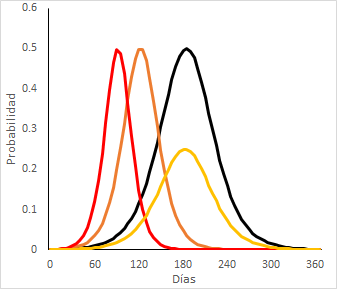
\includegraphics{img/graphs/graph-prob-avascular-3x4.png}}}
\subfigure[Etapa vascular $P_0^v = 2$.$5 \times 10^3$, $K_v = 6$.$3 \times 10^5$]{\scalebox{0.88}{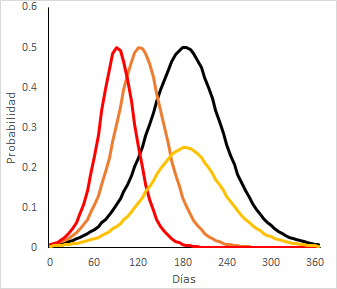
\includegraphics{img/graphs/graph-prob-vascular-3x4.png}}}
\end{center}\vspace*{-0.5cm}
\caption[Distribuciones de probabilidad de las funciones $\rho_a(n\Delta t)$ y $\rho_v(n\Delta t)$ que describen el crecimiento tumoral para distintos par\'ametros]{Distribuciones de probabilidad de las funciones $\rho_a(n\Delta t)$ y $\rho_v(n\Delta t)$ que describen el crecimiento tumoral durante las etapas avascular y vascular. (a) En negro $r_a=8$.$0 \times 10^{-4}$, $\Delta t = 53$; en naranja $r_a=8$.$0 \times 10^{-4}$, $\Delta t = 80$; en rojo $r_a=8$.$0 \times 10^{-4}$, $\Delta t = 107$; y en amarillo $r_a=4$.$0 \times 10^{-4}$, $\Delta t = 107$. (b) En negro $r_v=3$.$2 \times 10^{-6}$, $\Delta t = 9$.$4 \times 10^{3}$; en naranja $r_v=3$.$2 \times 10^{-6}$, $\Delta t = 1$.$4 \times 10^{4}$; en rojo $r_v=3$.$2 \times 10^{-6}$, $\Delta t = 1$.$9 \times 10^{4}$; y en amarillo $r_v=1$.$6 \times 10^{-6}$, $\Delta t = 1$.$9 \times 10^{4}$.}
\label{graph-probability-distribution-avascular}
\end{figure}

De estas gr\'aficas se puede inferir que seg\'un el modelo de crecimiento log\'istico la m\'axima velocidad de expansi\'on tumoral se presenta en los momentos centrales del lapso de tiempo correspondiente con cada etapa. Si se logra confirmar este hecho cl\'inicamente puede constituir una predici\'on importante ya que dadas dos observaciones del crecimiento tumoral que permitan determinar la velocidad de expansi\'on del tumor se puede determinar el momento en que transcurre su desarrollo y con este se puede determinar el tiempo que le toma alcanzar un tama\~no que ponga en peligro la vida del paciente.

\section{Par\'ametros de la asignaci\'on de estados iniciales y de los vectores de nutrientes}
\label{subsec-states-param}
Los par\'ametros de la asignaci\'on de estados iniciales se corresponden con la disposici\'on inicial de los estados en la simulaci\'on para representar un corte de tejido de las localizaciones donde se desarrolla el c\'ancer. El presente modelo est\'a orientado a representar el crecimiento de tumores que surgen en el epitelio correspondiente con el tipo de c\'ancer conocido como carcinoma. En la secci\'on anterior~\ref{subsec-network-param} se expuso que las simulaciones est\'an dirigidas a reproducir espec\'ificamente el carcinoma ductal infiltrante que surge en el epitelio que recubre los conductos mamarios, motivo por el que se conciben varios esquemas de asignaci\'on de estados iniciales: el primero para reproducir un corte de tejido gen\'erico donde se aprecien tres capas correspondientes con el lumen, el epitelio y el estroma, es decir, un corte que abarca tanto la superficie del \'organo como el interior; el segundo reproduce un corte de tejido correspondiente con una secci\'on del ducto mamario; mientras que el tercero reproduce un corte de tejido comprendido enteramente por estroma correspondiente al interior de un \'organo. Los esquemas I y II se utilizan fundamentalmente para representar el \'organo primario, mientras que el III para el \'organo secundario. En la figura~\ref{fig-initial-states-diagrams} se pueden apreciar dichos esquemas de asignaci\'on de estados iniciales.

\begin{figure}[!ht]
\begin{center}
\scalebox{0.5}{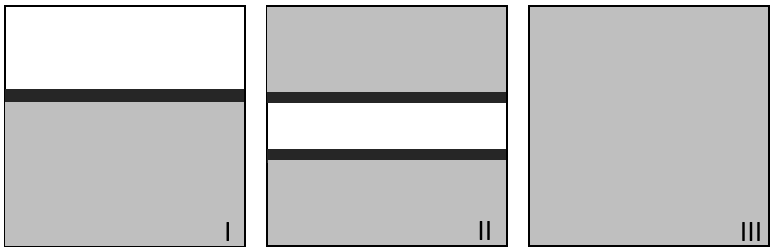
\includegraphics{img/fig-initial-states-diagrams.png}}
\end{center}\vspace*{-0.75cm}
\caption[Diagramas mostrando los esquemas de asignaci\'on de los estados iniciales]{Diagramas mostrando los esquemas de asignaci\'on de los estados iniciales. La asignaci\'on de colores es: blanco para el lumen, negro para el epitelio y gris para el estroma. }
\label{fig-initial-states-diagrams}
\end{figure}

Un elemento distintivo de la asignaci\'on de los estados iniciales es el tipo de tejido epitelial ya que el cuerpo humano cuenta con distintos tipos de epitelio en dependencia del \'organo representado, con disposiciones celulares y grosor distintos. En el ap\'endice~\ref{app-d} aparecen resumidos los distintos tipos de epitelios presentes en el cuerpo humano al igual que la figura~\ref{fig-epitheliums} que muestra los diagramas de estos tejidos~\cite{robins}. Dado que el aut\'omata celular reproduce las localizaciones que pueden ser ocupadas por c\'elulas cancer\'igenas se debe dividir el grosor del epitelio entre el tama\~no de una localizaci\'on representada. Una c\'elula del aut\'omata posee dimensiones aproximadas de $[0,3$.$5 \times 10^{-2}]mm \times [0,3$.$5 \times 10^{-2}]mm$ ya que se corresponden con las localizaciones que pueden ser ocupadas por una c\'elula cancer\'igena de un carcinoma ductal infiltrante. Los ductos mamarios constituyen estructuras tubulares con di\'ametro variable entre $0$.$1mm$ y $1mm$, revestidos por epitelio c\'ubico simple compuesto por una capa de c\'elulas de grosor equivalente al de una c\'elula cancer\'igena $3$.$5 \times 10^{-2}mm$. Por tanto la representaci\'on de este epitelio en el aut\'omata tambi\'en posee una \'unica capa de c\'elulas, es decir $o_e=1$. En los cuadros~\ref{table-states-params-1} y~\ref{table-states-params-2} aparecen recogidos los par\'ametros necesarios para la asignaci\'on de los estados iniciales de los esquemas I y II, exceptuando el III ya que est\'a compuesto enteramente por estroma.

\begin{table}[!ht]
\begin{center}
\scalebox{0.9}{\begin{tabular}{|p{2cm}|p{14.5cm}|} \hline
\emph{Par\'ametro} & \emph{Descripci\'on} \\\hline
\multicolumn{1}{|c|}{$o_l$} & Cantidad de capas del lumen.\\\hline
\multicolumn{1}{|c|}{$o_e$} & Cantidad de capas del epitelio. \\\hline
\multicolumn{1}{|c|}{$o_s$} & Cantidad de capas del estroma. Se determina como la cantidad de capas restantes en la red una vez que se disponen el lumen y el epitelio, es decir $o_s=s_y - (o_l + o_e)$.\\\hline
\multicolumn{1}{|c|}{$v_x^t$, $v_y^t$} & Coordenadas de la c\'elula cancer\'igena central del tumor inicial. La disposici\'on inicial del tumor se determina a partir de las coordenadas de esta c\'elula central. Se asume que la coordenada $v_y^t$ pertenece al siguiente rango de valores: $v_y^t \in [o_l, o_l + o_e]$, y generalmente $v_x^t = s_x/4$. \\\hline
\end{tabular}}\vspace*{-0.5cm}
\end{center}
\caption[Par\'ametros utilizados en la asignaci\'on de los estados iniciales a las c\'elulas del aut\'omata seg\'un el primer esquema]{Par\'ametros utilizados en la asignaci\'on de los estados iniciales a las c\'elulas del aut\'omata seg\'un el primer esquema.}
\label{table-states-params-1}
\end{table}

\begin{table}[!ht]
\begin{center}
\scalebox{0.9}{\begin{tabular}{|p{2cm}|p{14.5cm}|} \hline
\emph{Par\'ametro} & \emph{Descripci\'on} \\\hline
\multicolumn{1}{|c|}{$o_e$} & Cantidad de capas del epitelio.\\\hline
\multicolumn{1}{|c|}{$o_d$} & Coordenada de la l\'inea central del ducto mamario. Se extiende por los puntos $(v_x,o_d)$ para todo $v \in V(G)$.\\\hline
\multicolumn{1}{|c|}{$R^d$} & Radio del ducto mamario representado. Se itera por los v\'ertices $v \in V(G)$ de coordenadas $v = (v_x,v_y)$ y seg\'un la distancia euclideana~(Def. \ref{def-euclidean-distance}) entre dicho v\'ertice y su correspondiente en la l\'inea central del ducto mamario $v^d = (v_x,o_d)$ se le asigna uno de los estados correspondientes con c\'elulas normales: si $d_E(v,v^d) > R^d + o_e$ se asigna el estado $2$ correspondiente con el estroma; si $d_E(v,v^d) \in [R^d, R^d + o_e]$ se asigna el estado $1$ correspondiente con el epitelio; y si $d_E(v,v^d) < R^d$ se asigna el estado $0$ correspondiente con el lumen.\\\hline
\multicolumn{1}{|c|}{$v_x^t$, $v_y^t$} & Coordenadas de la c\'elula cancer\'igena central del tumor inicial. La disposici\'on inicial del tumor se determina a partir de las coordenadas de esta c\'elula central. Se asume que la coordenada $v_y^t$ pertenece a los siguientes rangos de valores: $v_y^t \in [o_d + R^d, o_d + (R^d + o_e)]$ y $v_y^t \in [ o_d - (R^d + o_e), o_d - R^d]$, y generalmente $v_x^t = s_x/4$. \\\hline
\end{tabular}}\vspace*{-0.5cm}
\end{center}
\caption[Par\'ametros utilizados en la asignaci\'on de los estados iniciales a las c\'elulas del aut\'omata seg\'un el segundo esquema]{Par\'ametros utilizados en la asignaci\'on de los estados iniciales a las c\'elulas del aut\'omata seg\'un el segundo esquema.}
\label{table-states-params-2}
\end{table}

En cuanto a las regiones y vectores de nutrientes del tejido, estos poseen el objetivo de dirigir tanto el crecimiento tumoral como la migraci\'on de c\'elulas cancer\'igenas hacia los tejidos con la presencia de una mayor vasculatura, y por lo tanto una mayor cantidad de nutrientes. Como se expuso en la secci\'on~\ref{subsec-celldiv}, generalmente el lumen y el epitelio deben contenerse en regiones que poseen un vector de nutrientes que apunte directamente hacia el estroma. A modo de ejemplo supongamos que se tiene un \'organo primario delimitado por las coordenadas $[0,1500] \times [0,1500]$ cuyo esquema de asignaci\'on de estados iniciales es el I correspondiente con un corte de tejido gen\'erico. En este caso se declaran dos regiones: 
\begin{itemize}
\item Regi\'on 1: Contiene el lumen y el epitelio, delimitada por los puntos $(0,0)$ y $(1500,o_l + o_e + \epsilon)$ donde $o_l + o_e$ es la cantidad de capas total existente entre el lumen y el epitelio, y $\epsilon$ es una cantidad adicional de capas correspondientes con las capas m\'as superficiales del estroma adyacentes al epitelio donde existe una variaci\'on de la concentraci\'on de nutrientes. Esta regi\'on puede denotarse como: $R_1 = \lbrace v~|~v \in V(G) : (0 \leq v_x < 1500) \wedge (0 \leq v_y < o_l + o_e + \epsilon) \rbrace$ y se vincula con el conjunto de vectores de concentraci\'on $B_{01}$ que contiene el vector $\overrightarrow{\nu}$ que tiene como puntos de origen y destino a $(0,0)$ y $(0,1)$, que indican un aumento de la concentraci\'on de nutrientes en direcci\'on al estroma.

\item Regi\'on 2: Contiene al resto del estroma, delimitada por los puntos $(0,o_l + o_e + \epsilon)$ y $(1500,1500)$ y que contiene efectivamente al resto del \'organo. En este caso dada la distribuci\'on regular de la vasculatura en el interior del tejido la concentraci\'on de nutrientes general es uniforme, por lo que no hay necesidad de definir ning\'un conjunto de vectores de concentraci\'on. 
\end{itemize}

En la figura~\ref{fig-initial-states-nutrients} se muestran diagramas de los esquemas de asignaci\'on de estados iniciales con la representaci\'on de las variaciones de concentraci\'on de nutrientes.

\begin{figure}[!ht]
\begin{center}
\scalebox{0.65}{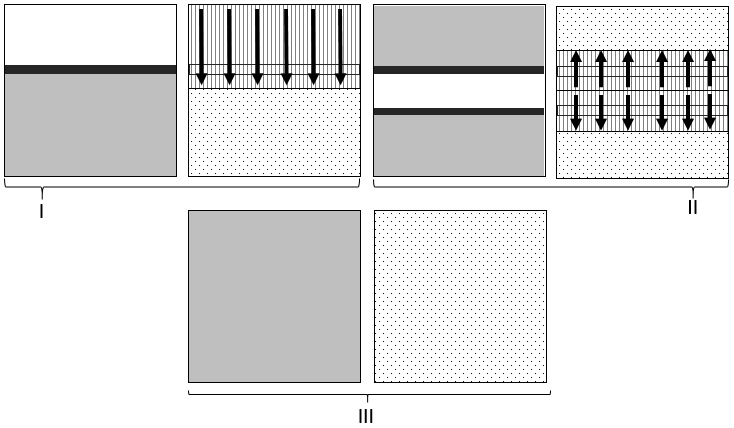
\includegraphics{img/fig-initial-states-nutrients.png}}
\end{center}\vspace*{-0.75cm}
\caption[Diagramas mostrando los esquemas de asignaci\'on de los estados iniciales con ejemplos de asignaci\'on de regiones y vectores de concentraci\'on de nutrientes]{Diagramas mostrando los esquemas de asignaci\'on de los estados iniciales con ejemplos de asignaci\'on de regiones y vectores de concentraci\'on de nutrientes. Posee la misma leyenda de colores de la figura~\ref{fig-initial-states-diagrams} para los diagramas izquierdos de cada par. Las regiones sombreadas con l\'ineas verticales poseen un vector de concentraci\'on de nutrientes con la direcci\'on especificada por la flecha, mientras que las regiones sombreadas con puntos indican una concentraci\'on uniforme de nutrientes. }
\label{fig-initial-states-nutrients}
\end{figure}

\section{Par\'ametros del modelo relacionados con la migraci\'on, invasi\'on y met\'astasis}
\label{subsec-model-param}
Los par\'ametros que se discuten en esta secci\'on se relacionan con las reglas y procedimientos de actualizaci\'on del aut\'omata celular encargados de reproducir los procesos de migraci\'on, invasi\'on y met\'astasis del c\'ancer. Se presentan en el cuadro~\ref{table-model-params} para una r\'apida referencia.

\begin{table}[!ht]
\begin{center}
\scalebox{0.9}{\begin{tabular}{|p{2cm}|p{14.5cm}|} \hline
\emph{Par\'ametro} & \emph{Descripci\'on} \\\hline
\multicolumn{1}{|c|}{$\mu_{mig}$} & Cantidad de movimientos tentativos que la c\'elula migratoria puede llevar a cabo en un instante de tiempo.\\\hline
\multicolumn{1}{|c|}{$\mu_{max}$} & Distancia m\'axima de migraci\'on.\\\hline
\multicolumn{1}{|c|}{$\xi_{sc}$} & Probabilidad de supervivencia de una c\'elula migratoria durante el transporte en el sistema circulatorio.\\\hline
\multicolumn{1}{|c|}{$\xi_{mic0}$,$\xi_{mic1}$} & Probabilidad de supervivencia de una micromet\'astasis.\\\hline
\multicolumn{1}{|c|}{$\psi_{mic0}$,$\psi_{mic1}$} & Probabilidad de colonizaci\'on de una micromet\'astasis.\\\hline
\multicolumn{1}{|c|}{$\eta_{mig}$} & Par\'ametro de ajuste de la probabilidad de transici\'on relacionada con la aparici\'on de c\'elulas migratorias.\\\hline
\multicolumn{1}{|c|}{$K_{mig}$} & Par\'ametro de ajuste de la probabilidad de transici\'on relacionada con la aparici\'on de c\'elulas migratorias.\\\hline
\multicolumn{1}{|c|}{$\eta_{mig}'$} & Par\'ametro de ajuste de la probabilidad de transici\'on relacionada con la muerte de c\'elulas migratorias durante su desplazamiento.\\\hline
\end{tabular}}\vspace*{-0.5cm}
\end{center}
\caption[Par\'ametros utilizados en el procedimiento de actualizaci\'on y en el ajuste de las reglas del aut\'omata celular]{Par\'ametros utilizados en el procedimiento de actualizaci\'on y en el ajuste de las reglas del aut\'omata celular.}
\label{table-model-params}
\end{table}

En~\cite{nurmenniemi} se expone que las c\'elulas migratorias de diversos tipos de carcinomas, entre los que se incluye el ductal infiltrante, son capaces de migrar desde la frontera del tumor hasta una distancia de $5$.$5 \times 10^{-1}mm$ en $14$ d\'ias como promedio. Si determinamos la velocidad de migraci\'on seg\'un los datos anteriores devuelve un promedio de $5$.$9 \times 10^{-2}mm$ en un d\'ia, valor cercano a las distancias entre c\'elulas del aut\'omata incluidas las diagonales que son de $3$.$5 \times 10^{-2}mm$ y $9$.$0 \times 10^{-2}mm$. Por tanto es razonable permitir en un lapso de $24$ horas que una c\'elula migratoria se desplace como m\'aximo una celda del aut\'omata en todas las direcciones, quedando el valor del par\'ametro $\mu_{mig} = 1$. Este par\'ametro es \'util si se desea ejecutar el aut\'omata celular con per\'iodos de tiempo diferentes para el crecimiento tumoral y para la migraci\'on; e.g. si el crecimiento tumoral se ejecuta con un per\'iodo de tiempo correspondiente con $24$ horas y la migraci\'on se eval\'ua con un per\'iodo de $48$ horas ser\'ia necesario hacer que $\mu_{mig} = 2$ para compensar. En~\cite{chaplain} se estima que la distancia m\'axima de migraci\'on de una c\'elula cancer\'igena est\'a entre $1mm$ y $10mm$. Dadas las dimensiones de una c\'elula en el aut\'omata, se pueden determinar la cantidad m\'axima de celdas que puede alejarse una c\'elula cancer\'igena de la frontera del tumor donde se originaron utilizando el dato anterior. Esto devuelve un valor entre $30$ y $300$ celdas aproximadamente, luego $\mu_{max} \in [30,300]$ con un valor promedio de $\mu_{max} = 165$ aproximadamente. De esta forma la cantidad de movimientos tentativos de una c\'elula se corresponden con la distancia m\'axima promedio de la migraci\'on siempre y cuando dicha c\'elula siempre se desplace en cada actualizaci\'on. 

En~\cite{luzzi} se estima experimentalmente que una c\'elula cancer\'igena solitaria que circule por el torrente sangu\'ineo tiene una probabilidad de supervivencia aproximada de $5$.$0 \times 10^{-4}$, mientras que en~\cite{aceto} se estima que los cl\'usteres de estas c\'elulas poseen una probabilidad de supervivencia entre $25$ y $50$ veces la supervivencia de una c\'elula solitaria, obteniendo un valor promedio de $1$.$9 \times 10^{-2}$. Dado que el presente modelo solo reproduce la migraci\'on de c\'elulas individuales se utiliza el valor de probabilidad de supervivencia determinado en~\cite{luzzi}, por tanto $\xi_{sc} = 5$.$0 \times 10^{-4}$. 

Seg\'un~\cite{kuhn,isogenic} los destinos m\'as frecuentes de las met\'astasis del carcinoma ductal infiltrante lo constituyen los huesos, pulmones e h\'igado en ese orden, en un $60\%$, $34\%$ y $20\%$ de los casos, mientras que las met\'astasis en la propia mama son muy poco frecuentes. Este hecho se puede interpretar de acuerdo a la teor\'ia de la semilla y el sustrato como un indicador de la hostilidad del entorno del \'organo hacia las c\'elulas cancer\'igenas, y por tanto puede utilizarse como v\'ia para determinar los par\'ametros $\xi_{mic}$ y $\psi_{mic}$. 

Como se expuso en la secci\'on~\ref{subsec-migrant}, la elecci\'on de los par\'ametros de ajuste $\eta_{mig}$ y $K_{mig}$ permite representar la aparici\'on de c\'elulas migratorias adecuadamente. En~\cite{kansal3} el valor de esta probabilidad de aparici\'on de c\'elulas migratorias se establece como un valor constante igual a $0$.$05$ en toda la simulaci\'on para obtener ramas invasivas poco densas, lo cual nos otorga una medida para ajustar nuestra funci\'on de probabilidad. Si se desea reproducir un c\'ancer con un alto nivel migratorio se precisa establecer un valor de probabilidad m\'as alto. En la gr\'afica~\ref{graph-probability-aparition} se muestran las distribuciones de probabilidad de la funci\'on $\rho_2(n_i \rightarrow 4)$~(\ref{eq-migrant-2}) que describe la aparici\'on de c\'elulas migratorias tanto en la frontera del tumor como en el interior del mismo para distintos par\'ametros. Estas gr\'aficas muestran que a medida que avanza el tiempo la probabilidad de que surjan c\'elulas migratorias se ve en aumento, tal y como ocurre con el proceso de acumulaci\'on de mutaciones. Mientras mayor es la cantidad de errores en el c\'odigo gen\'etico mayor es la agresividad de las c\'elulas cancer\'igenas, tomando la consideraci\'on de que las c\'elulas migratorias presentan una peligrosidad mayor que las c\'elulas que permanecen adheridas al tumor.

\begin{figure}[!ht]
\begin{center}
\subfigure[$K_{mig}=3$.$2 \times 10^{5}$]{\scalebox{0.88}{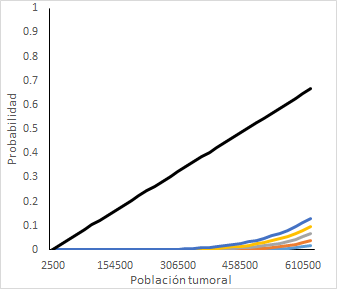
\includegraphics{img/graphs/graph-prob-aparition-1.png}}}
\subfigure[$K_{mig}=2$.$1 \times 10^{5}$]{\scalebox{0.88}{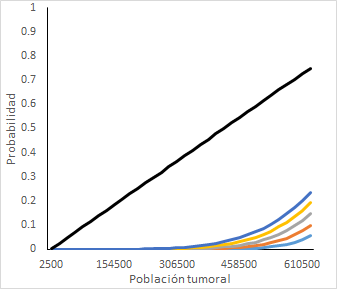
\includegraphics{img/graphs/graph-prob-aparition-2.png}}}
\subfigure[$K_{mig}=1$.$6 \times 10^{5}$]{\scalebox{0.88}{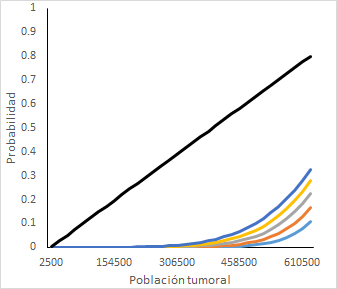
\includegraphics{img/graphs/graph-prob-aparition-3.png}}}
\subfigure[$K_{mig}=1$.$3 \times 10^{5}$]{\scalebox{0.88}{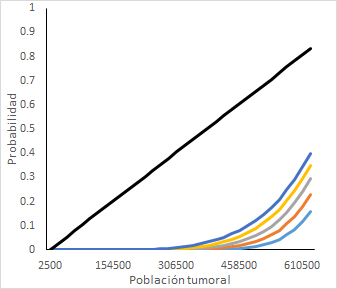
\includegraphics{img/graphs/graph-prob-aparition-4.png}}}
\end{center}\vspace*{-0.5cm}
\caption[Distribuciones de probabilidad de la funci\'on $\rho_2(n_i \rightarrow 4)$ que describe la aparici\'on de c\'elulas migratorias para distintos par\'ametros]{Distribuciones de probabilidad de la funci\'on $\rho_2(l \rightarrow 4)$ que describe la aparici\'on de c\'elulas migratorias. (a,b,c,d) En azul claro $\eta_{mig}=0$.$1$; en naranja $\eta_{mig}=0$.$125$; en gris $\eta_{mig}=0$.$15$; en amarillo $\eta_{mig}=0$.$175$; en azul oscuro $\eta_{mig}=0$.$2$; y en negro $\eta_{mig}=1$.}
\label{graph-probability-aparition}
\end{figure}

El par\'ametro de ajuste $\eta_{mig}'$ de la regla que determina la muerte de una c\'elula migratoria durante su avance por el estroma posee un funcionamiento similar a $\eta_{mig}$. En la gr\'afica~\ref{graph-probability-migration} se muestran las distribuciones de probabilidad de la funci\'on $\rho_4(\mu(v,n) \rightarrow 2)$~(\ref{eq-rho-4}) que describe la muerte de c\'elulas migratorias en su avance por el estroma. En estas gr\'aficas se muestra que una c\'elula migratoria a medida que permanece una mayor cantidad de tiempo en el estroma aumenta la probabilidad de que termine su existencia debido a su eliminaci\'on por parte del sistema inmunitario o de que ocurra por causas naturales como estr\'es mec\'anico, falta de nutrici\'on o por ausencia de se\~nales del entorno.

\begin{figure}[!ht]
\begin{center}
\subfigure[$\mu_{max}=150$]{\scalebox{0.88}{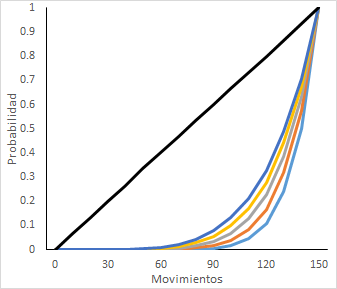
\includegraphics{img/graphs/graph-prob-migrant-1.png}}}
\subfigure[$\mu_{max}=300$]{\scalebox{0.88}{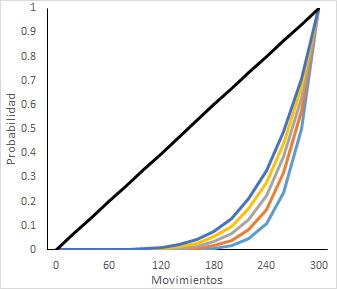
\includegraphics{img/graphs/graph-prob-migrant-2.png}}}
\end{center}\vspace*{-0.5cm}
\caption[Distribuciones de probabilidad de la funci\'on $\rho_4(\mu(v,n) \rightarrow 2)$ que describe la muerte de c\'elulas migratorias en su avance por el estroma para distintos par\'ametros]{Distribuciones de probabilidad de la funci\'on $\rho_4(\mu(v,n) \rightarrow 2)$ que describe la muerte de c\'elulas migratorias en su avance por el estroma para distintos par\'ametros. (a,b) En azul claro $\eta_{mig}'=0$.$1$; en naranja $\eta_{mig}'=0$.$125$; en gris $\eta_{mig}'=0$.$15$; en amarillo $\eta_{mig}'=0$.$175$; en azul oscuro $\eta_{mig}'=0$.$2$; y en verde $\eta_{mig}'=1$. }
\label{graph-probability-migration}
\end{figure}

\section{Escala de la simulaci\'on}
\label{subsec-scale-param}
En las secciones anteriores se ha descrito los procedimientos y an\'alisis que se llevan a cabo para obtener los par\'ametros del modelo necesarios para su ejecuci\'on. Estos par\'ametros se corresponden con una simulaci\'on en escala real, donde una c\'elula en la simulaci\'on equivale a una c\'elula en vida real. Una simulaci\'on de estas dimensiones puede tomar un lapso de tiempo enorme en concluir, haciendo que tareas como la obtenci\'on de datos estad\'isticos y validaci\'on del modelo presenten dificultades. Por tanto se opta por escalar los par\'ametros del modelo seg\'un el tama\~no de una celda del aut\'omata. En la escala real, o escala $1:1$, una celda del aut\'omata posee dimensiones $[0,3$.$5 \times 10^{-2}]mm \times [0, 3$.$5 \times 10^{-2}]mm$ correspondientes con el tama\~no aproximado que posee una c\'elula cancer\'igena de un carcinoma ductal infiltrante como se mostr\'o en la secci\'on~\ref{subsec-network-param}. La idea central es multiplicar el tama\~no de las celdas del aut\'omata por un valor de escala entero haciendo que cada celda del aut\'omata contenga una cantidad variable de c\'elulas reales, e.g. si se utiliza la escala $1:2$ las dimensiones de una celda del aut\'omata son $[0,7$.$0 \times 10^{-2}]mm \times [0, 7$.$0 \times 10^{-2}]mm$ correspondientes con $4$ c\'elulas reales. De esta forma el comportamiento de las c\'elulas reales contenidas en una misma celda se determina mediante una \'unica aplicaci\'on de las reglas del aut\'omata, reduciendo la cantidad de c\'alculos requeridos. 

Este procedimiento trae un problema relacionado con la representaci\'on de procesos como el crecimiento tumoral o la migraci\'on cancer\'igena. El m\'aximo incremento posible de la poblaci\'on de un tumor de un instante de tiempo $n$ a un instante $n+1$ lo constituyen las c\'elulas normales vecinas a la frontera del propio tumor. Dado que la influencia del estado de una c\'elula en sus vecinas est\'a limitada por el radio de la configuraci\'on de vecindad $R=\sqrt{2}$, como se expuso en la secci\'on~\ref{subsec-watts-2}, solo las c\'elulas normales que se sit\'uen a una distancia menor o igual a $R$ pueden ser desplazadas por el crecimiento tumoral. Esto se traduce en que un tumor representado por el aut\'omata puede incrementar su radio desde su centroide hasta la frontera exactamente la misma medida que posee una celda del mismo. Si se utiliza la escala $1:1$ en un lapso de $24$ horas el tumor puede incrementar cualquiera de sus radios en la medida de una celda, que en este caso se corresponde con la medida de una c\'elula real, es decir $3$.$5 \times 10^{-2}mm$. Pero en una escala mayor las celdas del aut\'omata poseen medidas mayores por lo que contienen una mayor cantidad de c\'elulas reales. Para lograr que los incrementos en el radio tumoral sean los correctos se debe incrementar el lapso de tiempo que ocurre entre instantes de tiempo y modificar adecuadamente los valores de $r$ y $\Delta t$. En la figura~\ref{fig-scales-1} se muestran ejemplos de varias escalas y el lapso de tiempo que se debe tomar para una representaci\'on adecuada. Se puede inferir que el lapso de tiempo se debe escalar la misma magnitud que las dimensiones de una celda del aut\'omata, e.g. si se utiliza la escala $1:2$ es necesario que el tiempo transcurrido entre los instantes $n$ y $n+1$ sea equivalente a $48$ horas que es el tiempo m\'inimo necesario para que una celda del aut\'omata sea ocupada por el tumor. Se asume que una celda del aut\'omata cuyo estado se corresponda con el de un tumor~(estado $3$) o el de una micromet\'astasis~(estado $4$) se encuentra totalmente ocupado por c\'elulas de esos tipos. N\'otese que este an\'alisis no posee contradicciones con lo expresado en la secci\'on~\ref{subsec-celldiv} sobre el sesgo direccional del crecimiento tumoral basado en la velocidad de expansi\'on.

\begin{figure}[!ht]
\begin{center}
\subfigure[Escala $1:1$]{\scalebox{0.67}{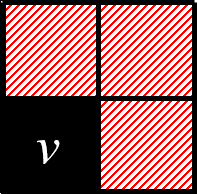
\includegraphics{img/fig-scales.png}}}
\subfigure[Escala $1:2$]{\scalebox{0.67}{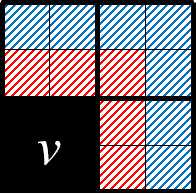
\includegraphics{img/fig-scales-1.png}}}
\subfigure[Escala $1:3$]{\scalebox{0.67}{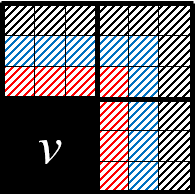
\includegraphics{img/fig-scales-2.png}}}
\end{center}\vspace*{-0.5cm}
\caption[Representaci\'on de distintas escalas del aut\'omata celular]{Representaci\'on de distintas escalas del aut\'omata celular y de los lapsos de tiempo necesarios para que un tumor se expanda satisfactoriamente a trav\'es del espacio mostrado. La celda $v$ representa una c\'elula tumoral que intenta expandirse a las celdas restantes. Las \'areas sombreadas muestran el tiempo m\'inimo necesario para que el tumor ocupe dichas c\'elulas seg\'un la escala utilizada. El color rojo se corresponde con $24$ horas, el color azul con $48$ horas y el negro con $72$ horas. (a) Las dimensiones de una celda del aut\'omata equivalen al de una c\'elula cancer\'igena $3$.$5 \times 10^{-2}mm$. (b) Las dimensiones de una celda del aut\'omata es el doble de una c\'elula cancer\'igena $7$.$0 \times 10^{-2}mm$ por lo que cada celda contiene $4$ c\'elulas. (c) Las dimensiones de una celda del aut\'omata es el triple de una c\'elula cancer\'igena $1$.$05 \times 10^{-1}mm$ por lo que cada celda contiene $9$ c\'elulas.}
\label{fig-scales-1}
\end{figure}

\begin{table}[!ht]
\begin{center}
\scalebox{1}{\begin{tabular}{|l|r|r|r|r|} \hline
\multicolumn{2}{|c|}{\emph{Par\'ametros}} & \multicolumn{3}{|c|}{\emph{Escalas}} \\\cline{3-5}
\multicolumn{2}{|c|}{} & \multicolumn{1}{|c|}{$1:1$} & \multicolumn{1}{|c|}{$1:2$} & \multicolumn{1}{|c|}{$1:3$} \\\hline
\emph{Dimensiones del espacio} & $s_x$ & $3000$ & $1500$ & $1000$ \\\cline{2-5}
                               & $s_y$ & $1500$ & $750$ & $500$ \\\hline
\multicolumn{2}{|l|}{\emph{Tiempo entre generaciones en horas}} & $24$ & $48$ & $72$ \\\hline
\multicolumn{2}{|l|}{\emph{C\'elulas contenidas en una celda}} & $1$ & $4$ & $9$ \\\hline

\emph{Poblaci\'on inicial avascular}& $P_0^a$ & $1$ & $1$ & $1$ \\\hline

\emph{Capacidad de carga avascular o}& $K_a$(m\'in) & $6$.$25 \times 10^2$ & $1$.$563 \times 10^2$ & $6$.$944 \times 10^1$ \\\cline{2-5}
\emph{poblaci\'on inicial vascular} & $K_a$(m\'ax) & $4$.$444 \times 10^3$ & $1$.$111 \times 10^3$ & $4$.$938 \times 10^2$ \\\cline{2-5}
									& $K_a$(med) & $2$.$535 \times 10^3$ & $4$.$592 \times 10^2$ & $2$.$222 \times 10^2$ \\\hline

\emph{Capacidad de carga vascular} & $K_v$(m\'in) & $2$.$5 \times 10^5$ & $6$.$25 \times 10^4$ & $2$.$778 \times 10^4$ \\\cline{2-5}
                                   & $K_v$(m\'ax) & $1$.$0 \times 10^6$ & $2$.$5 \times 10^5$ & $1$.$111 \times 10^5$ \\\cline{2-5}
                                   & $K_v$(med) & $6$.$25 \times 10^5$ & $1$.$276 \times 10^5$ & $5$.$556 \times 10^4$ \\\hline

\emph{Movimientos tentativos} & $\mu_{mig}$ & $1$ & $1$ & $1$\\\hline

\emph{Distancia m\'axima de la migraci\'on} & $\mu_{max}$ & $165$ & $84$ & $55$ \\\hline
\end{tabular}}\vspace*{-0.5cm}
\end{center}
\caption[Escalas consideradas para su utilizaci\'on en el aut\'omata celular]{Escalas consideradas para su utilizaci\'on en el aut\'omata celular. Se muestran varios par\'ametros del modelo corregidos para dichas escalas.}
\label{table-reescale}
\end{table} 

El an\'alisis seguido para el crecimiento tumoral se puede realizar de igual forma con la migraci\'on, obteni\'endose la misma conclusi\'on. En la secci\'on~\ref{subsec-model-param} se expuso que una c\'elula migratoria puede desplazarse aproximadamente $3$.$9 \times 10^{-2}mm$ en $24$ horas, que se corresponde con una celda del aut\'omata en la escala real. Si utilizamos un tama\~no mayor para las celdas del aut\'omata una c\'elula migratoria deber\'a tomarle m\'as tiempo para avanzar desde una celda hacia la siguiente. Luego el lapso de tiempo transcurrido entre los instantes de tiempo $n$ y $n+1$ debe aumentar para reproducir de forma adecuada dicho movimiento. 

El otro problema que presenta el uso de escalas gira en torno a las cantidades de c\'elulas cancer\'igenas que penetran el torrente sangu\'ineo, ya sea como la culminaci\'on de la migraci\'on o que esta penetraci\'on ocurra desde el interior del propio tumor. En escala real la migraci\'on y la penetraci\'on del torrente sangu\'ineo desde los capilares del tumor se lleva a cabo por c\'elulas individuales, pero si se utiliza una escala se establece que el comportamiento de varias c\'elulas se determina mediante la aplicaci\'on de una misma regla. Para el crecimiento tumoral se asume que la cantidad de c\'elulas contenidas en una celda del aut\'omata se corresponde con la cantidad m\'axima que puede contener. Esta suposici\'on se sostiene en el hecho que el interior del tumor contin\'ua desarroll\'andose cubriendo los espacios existentes. Con respecto a las c\'elulas migratorias se asigna un valor entero aleatorio perteneciente al intervalo $[1,max]$ a cada c\'elula que surge de este tipo, correspondiente con la cantidad de c\'elulas contenidas en dicha celda del aut\'omata, donde $max$ es la m\'axima cantidad de c\'elulas que puede contener una celda, e.g en la escala $1:2$ el valor de $max=4$. Este mecanismo se implementa de forma similar en el algoritmo encargado de reproducir la intravasaci\'on desde el interior del tumor de c\'elulas migratorias. En el cuadro~\ref{table-reescale} se muestran varios par\'ametros del modelo de aut\'omatas que se han obtenido en las secciones anteriores corregidos para su utilizaci\'on con las escalas consideradas. Despu\'es de sucesivas pruebas se descarta la posibilidad de utilizar las escalas $1:1$ y $1:2$ debido a la carga computacional que presentan. 